%\VignetteIndexEntry{Introduction to the dataRetrieval package}
%\VignetteDepends{}
%\VignetteSuggests{}
%\VignetteImports{}
%\VignettePackage{}

\documentclass[a4paper,11pt]{article}

\usepackage{amsmath}
\usepackage{times}
\usepackage{hyperref}
\usepackage[numbers, round]{natbib}
\usepackage[american]{babel}
\usepackage{authblk}
\renewcommand\Affilfont{\itshape\small}
\usepackage{Sweave}
\renewcommand{\topfraction}{0.85}
\renewcommand{\textfraction}{0.1}
\usepackage{graphicx}


\textwidth=6.2in
\textheight=8.5in
\parskip=.3cm
\oddsidemargin=.1in
\evensidemargin=.1in
\headheight=-.3in

%------------------------------------------------------------
% newcommand
%------------------------------------------------------------
\newcommand{\scscst}{\scriptscriptstyle}
\newcommand{\scst}{\scriptstyle}
\newcommand{\Robject}[1]{{\texttt{#1}}}
\newcommand{\Rfunction}[1]{{\texttt{#1}}}
\newcommand{\Rclass}[1]{\textit{#1}}
\newcommand{\Rpackage}[1]{\textit{#1}}
\newcommand{\Rexpression}[1]{\texttt{#1}}
\newcommand{\Rmethod}[1]{{\texttt{#1}}}
\newcommand{\Rfunarg}[1]{{\texttt{#1}}}

\begin{document}
\Sconcordance{concordance:dataRetrieval.tex:dataRetrieval.Rnw:%
1 126 1 49 0 1 7 15 1 1 14 55 1 3 0 36 1 2 0 11 1 24 %
0 24 1 3 0 23 1 3 0 6 1 7 0 18 1 3 0 25 1 1 0 17 1 9 %
0 6 1 7 0 21 1 8 0 16 1 2 0 11 1 23 0 21 1 9 0 20 1 3 %
0 6 1 17 0 27 1 6 0 11 1 9 0 15 1 20 0 21 1 4 0 21 1 %
4 0 17 1 7 0 22 1 8 0 19 1 4 0 9 1 4 0 78 1 1 2 9 1 1 %
4 4 1 20 0 44 1 4 0 32 1 4 0 21 1 4 0 21 1 37 0 13 1 %
9 0 95 1 4 0 9 1 12 0 13 1 4 0 14 1 4 0 5 1 4 0 23 1 %
18 0 8 1 4 0 55 1}


%------------------------------------------------------------
\title{Introduction to the dataRetrieval package}
%------------------------------------------------------------
\author[1]{Laura De Cicco}
\author[1]{Robert Hirsch}
\affil[1]{United States Geological Survey}



\maketitle
\tableofcontents

%------------------------------------------------------------
\section{Introduction to dataRetrieval}
%------------------------------------------------------------ 
The dataRetrieval package was created to simplify the process of getting hydrologic data in the R enviornment. It has been specifically designed to work seamlessly with the EGRET package: Exploration and Graphics for RivEr Trends (EGRET). See: \url{https://github.com/USGS-R/EGRET/wiki} for information on EGRET.

There is a plethora of hydrological data available on the web. This package is designed specifically to load United States Geological Survey (USGS) hydrologic data to the R enviornment. This includes daily values, real-time (unit values), site information, and water quality sample data. 

For information on getting started in R, downloading and installing the package, see Appendix 1: Getting Started.


%------------------------------------------------------------
\section{USGS Web Retrieval Examples}
%------------------------------------------------------------ 
In this section, we will run through 5 examples, documenting how to get raw data from the web. This includes historical daily values, real-time current values, water quality data, site information, and measured parameter information. We will use the Choptank River near Greensboro, MD as an example.  The site-ID for this gage station is 01491000. Daily discharge measurements are available as far back as 1948.  Additionally, forms of nitrate have been measured dating back to 1964. The functions/examples in this section are for raw data retrieval.  This may or may not be the easiest data to work with.  In the next section, we will use functions that retrieve and process the data in a dataframe that may prove more friendly for R analysis.

%------------------------------------------------------------
\subsection{USGS Web Retrieval Introduction}
%------------------------------------------------------------
The United States Geological Survey organizes their hydrological data in fairly standard structure.  Gage stations are located throughout the United States, each station has a unique ID.  Often (but not always), these ID's are 8 digits.  The first step to finding data is discoving this 8-digit ID. One potential tool for discovering data is Environmental Data Discovery and Transformation (EnDDaT): \url{http://cida.usgs.gov/enddat/}.  Follow the example in the User's Guide to learn how to discover USGS stations and available data from any location in the United States. Essentially, you can create a Project Location on the map, set a bounding box (in miles), then search for USGS Time Series and USGS Water Quality Data. Locations, ID's, available data, and available time periods will load on the map and appropriate tabs.

Once the site-ID is known, the next required input for USGS data retrievals is the 'parameter code'.  This is a 5-digit code that specifies what measured paramater is being requested.  A complete list of possible USGS parameter codes can be found at \href{http://nwis.waterdata.usgs.gov/usa/nwis/pmcodes?radio_pm_search=param_group&pm_group=All+--+include+all+parameter+groups&pm_search=&casrn_search=&srsname_search=&format=html_table&show=parameter_group_nm&show=parameter_nm&show=casrn&show=srsname&show=parameter_units}{nwis.waterdata.usgs.gov}. Not every station will measure all parameters. The following is a list of commonly measured parameters:



% latex table generated in R 2.15.2 by xtable 1.7-0 package
% Thu Feb 14 17:09:15 2013
\begin{table}[ht]
\begin{center}
\caption{Commonly found USGS Parameter Codes}
\begin{tabular}{rll}
  \hline
 & pCode & shortName \\ 
  \hline
1 & 00060 & Discharge [cfs] \\ 
  2 & 00065 & Gage height [ft] \\ 
  3 & 00010 & Temperature [C] \\ 
  4 & 00045 & Precipitation [in] \\ 
  5 & 00400 & pH \\ 
   \hline
\end{tabular}
\end{center}
\end{table}
For real-time data, the parameter code and site ID will suffice.  The USGS stores historical data as daily values however.  The statistical process used to store the daily data is the final requirement for daily value retrievals.  A 5-digit 'stat code' specifies the requested processing.  A complete list of possible USGS stat codes can be found here:

\url{http://nwis.waterdata.usgs.gov/nwis/help/?read_file=stat&format=table}

The most common stat codes are:
% latex table generated in R 2.15.2 by xtable 1.7-0 package
% Thu Feb 14 17:09:16 2013
\begin{table}[ht]
\begin{center}
\caption{Commonly found USGS Stat Codes}
\begin{tabular}{rll}
  \hline
 & StatCode & shortName \\ 
  \hline
1 & 00001 & Maximum \\ 
  2 & 00002 & Minimum \\ 
  3 & 00003 & Mean \\ 
  4 & 00008 & Median \\ 
   \hline
\end{tabular}
\end{center}
\end{table}

%------------------------------------------------------------
\subsection{USGS Site Information Retrievals}
%------------------------------------------------------------
To obtain all of the available site information, use the getSiteFileData function:
\begin{Schunk}
\begin{Sinput}
> library(dataRetrieval)
> # Site ID for Choptank River near Greensboro, MD
> siteNumber <- "01491000" 
> ChoptankInfo <- getSiteFileData(siteNumber)
\end{Sinput}
\end{Schunk}


% latex table generated in R 2.15.2 by xtable 1.7-0 package
% Thu Feb 14 17:09:16 2013
\begin{tabular}{rllll}
  \hline
 & ColumnNames & ColumnNames.1 & ColumnNames.2 & ColumnNames.3 \\ 
  \hline
1 & agency.cd & dec.coord.datum.cd & alt.datum.cd & reliability.cd \\ 
  2 & site.no & district.cd & huc.cd & gw.file.cd \\ 
  3 & station.nm & state.cd & basin.cd & nat.aqfr.cd \\ 
  4 & site.tp.cd & county.cd & topo.cd & aqfr.cd \\ 
  5 & lat.va & country.cd & instruments.cd & aqfr.type.cd \\ 
  6 & long.va & land.net.ds & construction.dt & well.depth.va \\ 
  7 & dec.lat.va & map.nm & inventory.dt & hole.depth.va \\ 
  8 & dec.long.va & map.scale.fc & drain.area.va & depth.src.cd \\ 
  9 & coord.meth.cd & alt.va & contrib.drain.area.va & project.no \\ 
  10 & coord.acy.cd & alt.meth.cd & tz.cd & queryTime \\ 
  11 & coord.datum.cd & alt.acy.va & local.time.fg &  \\ 
   \hline
\end{tabular}\\*

Pulling out a specific example piece of information, in this case station name can be done as follows:
\begin{Schunk}
\begin{Sinput}
> ChoptankInfo$station.nm
\end{Sinput}
\begin{Soutput}
[1] "CHOPTANK RIVER NEAR GREENSBORO, MD"
\end{Soutput}
\end{Schunk}
Site information is obtained from \url{http://waterservices.usgs.gov/rest/Site-Test-Tool.html}

%------------------------------------------------------------
\subsection{USGS Parameter Information Retrievals}
%------------------------------------------------------------
To obtain all of the available information concerning a measured parameter, use the getParameterInfo function:
\begin{Schunk}
\begin{Sinput}
> # Using defaults:
> parameterCd <- "00618" 
> parameterINFO <- getParameterInfo(parameterCd)
> colnames(parameterINFO)
\end{Sinput}
\begin{Soutput}
[1] "parameter_cd"       "parameter_group_nm" "parameter_nm"      
[4] "casrn"              "srsname"            "parameter_units"   
\end{Soutput}
\end{Schunk}

Pulling out a specific example piece of information, in this case station name can be done as follows:
\begin{Schunk}
\begin{Sinput}
> parameterINFO$parameter_nm
\end{Sinput}
\begin{Soutput}
[1] "Nitrate, water, filtered, milligrams per liter as nitrogen"
\end{Soutput}
\end{Schunk}
Parameter information is obtained from \url{http://nwis.waterdata.usgs.gov/nwis/pmcodes/}

%------------------------------------------------------------
\subsection{USGS Daily Value Retrievals}
%------------------------------------------------------------
To obtain historic daily records of USGS data, use the retrieveNWISData function. The arguments for this function are siteNumber, parameterCd, startDate, endDate, statCd, and a logical (true/false) interactive. There are 2 default argument: statCd defaults to "00003" and interactive defaults to TRUE.  If you want to use the default values, you do not need to list them in the function call. Setting the 'interactive' option to true will walk you through the function. It might make more sense to run large batch collections with the interactive option set to FALSE. 

The dates (start and end) need to be in the format "YYYY-MM-DD".  Setting the start date to "" will indicate to the program to ask for the earliest date, setting the end date to "" will ask for the latest available date.

\begin{Schunk}
\begin{Sinput}
> # Using defaults:
> siteNumber <- "01491000"
> parameterCd <- "00060"  # Discharge in cubic feet per second
> startDate <- ""  # Will request earliest date
> endDate <- "" # Will request latest date
> discharge <- retrieveNWISData(siteNumber, parameterCd, startDate, endDate)
\end{Sinput}
\end{Schunk}

A dataframe is returned that looks like the following:
\begin{Schunk}
\begin{Soutput}
  agency_cd  site_no   datetime X02_00060_00003 X02_00060_00003_cd
1      USGS 01491000 1948-01-01             190                  A
2      USGS 01491000 1948-01-02             900                  A
3      USGS 01491000 1948-01-03             480                  A
4      USGS 01491000 1948-01-04             210                  A
5      USGS 01491000 1948-01-05             210                  A
6      USGS 01491000 1948-01-06             220                  A
\end{Soutput}
\end{Schunk}

The variable datetime is automatically imported as a Date. Each requested parameter has a value and remark code column.  The names of these columns depend on the requested parameter and stat code combinations. USGS remark codes are often "A" (approved for publication) or "P" (provisional data subject to revision). A more complete list of remark codes can be found here:
\url{http://waterdata.usgs.gov/usa/nwis/help?codes_help}

Another example that doesn't use the defaults would be a request for mean and maximum daily temperature and discharge in early 2012:
\begin{Schunk}
\begin{Sinput}
> # Using defaults:
> siteNumber <- "01491000" 
> parameterCd <- "00010,00060"  # Temperature and discharge
> statCd <- "00001,00003"  # Mean and maximum
> startDate <- "2012-01-01"
> endDate <- "2012-06-30"
> temperatureAndFlow <- retrieveNWISData(siteNumber, parameterCd, 
                   startDate, endDate, StatCd=statCd,interactive=FALSE)
\end{Sinput}
\end{Schunk}

Daily data is pulled from \url{http://waterservices.usgs.gov/rest/DV-Test-Tool.html}. 

An example of plotting the above data (Figure 1):

\begin{Schunk}
\begin{Sinput}
> with(temperatureAndFlow, plot(
   datetime, X01_00010_00003,
   xlab="Date",ylab="Temperature [C]"
   ))
> par(new=TRUE)
> with(temperatureAndFlow, plot(
   datetime, X02_00060_00003,
   col="red",type="l",xaxt="n",yaxt="n",xlab="",ylab="",axes=FALSE
   ))
> axis(4,col="red",col.axis="red")
> mtext("Discharge [cfs]",side=4,line=3,col="red")
\end{Sinput}
\end{Schunk}
\newpage

\begin{figure}
\begin{center}
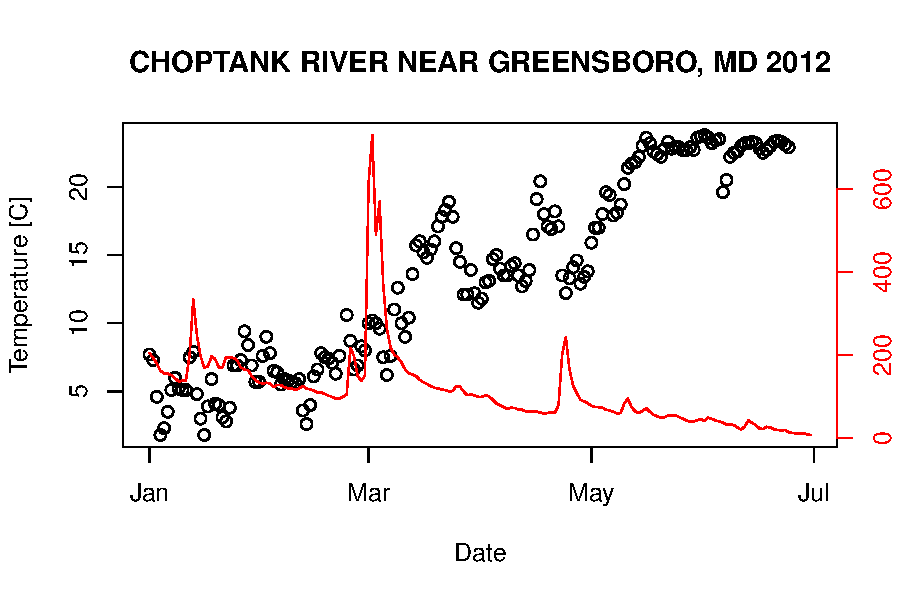
\includegraphics{dataRetrieval-fig1}
\end{center}
\caption{Temperature and discharge plot of Choptank River in 2012.}
\end{figure}


There are occasions where NWIS values are not reported as numbers, instead there might be text describing a certain event such as "Ice".  Any value that cannot be converted to a number will be reported as NA in this package.


%------------------------------------------------------------
\subsection{USGS Unit Value Retrievals}
%------------------------------------------------------------
We can also get real-time, instantaneous measurements using the retrieveUnitNWISData function:
\begin{Schunk}
\begin{Sinput}
> siteNumber <- "01491000" # Site ID for Choptank River near Greensboro, MD
> parameterCd <- "00060"  # Discharge in cubic feet per second
> startDate <- as.character(Sys.Date()-1) # Yesterday 
>   # (or, the day before the dataRetrieval package was built)
> endDate <- as.character(Sys.Date()) # Today 
>   # (or, the day the dataRetrieval package was built)
> 
> dischargeToday <- retrieveUnitNWISData(siteNumber, parameterCd, 
         startDate, endDate)
\end{Sinput}
\end{Schunk}
Which produces the following dataframe:
\begin{Schunk}
\begin{Soutput}
  agency_cd  site_no            datetime tz_cd X02_00060 X02_00060_cd
1      USGS 01491000 2013-02-13 00:00:00   EST       209            P
2      USGS 01491000 2013-02-13 00:15:00   EST       209            P
3      USGS 01491000 2013-02-13 00:30:00   EST       211            P
4      USGS 01491000 2013-02-13 00:45:00   EST       209            P
5      USGS 01491000 2013-02-13 01:00:00   EST       206            P
6      USGS 01491000 2013-02-13 01:15:00   EST       206            P
\end{Soutput}
\end{Schunk}

Note that time now becomes important, so the variable datetime is a POSIXct, and the time zone is included in a separate column. Data is pulled from \url{http://waterservices.usgs.gov/rest/IV-Test-Tool.html}. There are occasions where NWIS values are not reported as numbers, instead a common example is "Ice".  Any value that cannot be converted to a number will be reported as NA in this package.

A simple plotting example is shown in Figure 2:
\begin{Schunk}
\begin{Sinput}
> with(dischargeToday, plot(
   datetime, X02_00060,
   ylab="Discharge [cfs]",xlab=""
   ))
\end{Sinput}
\end{Schunk}
\newpage

\begin{figure}
\begin{center}
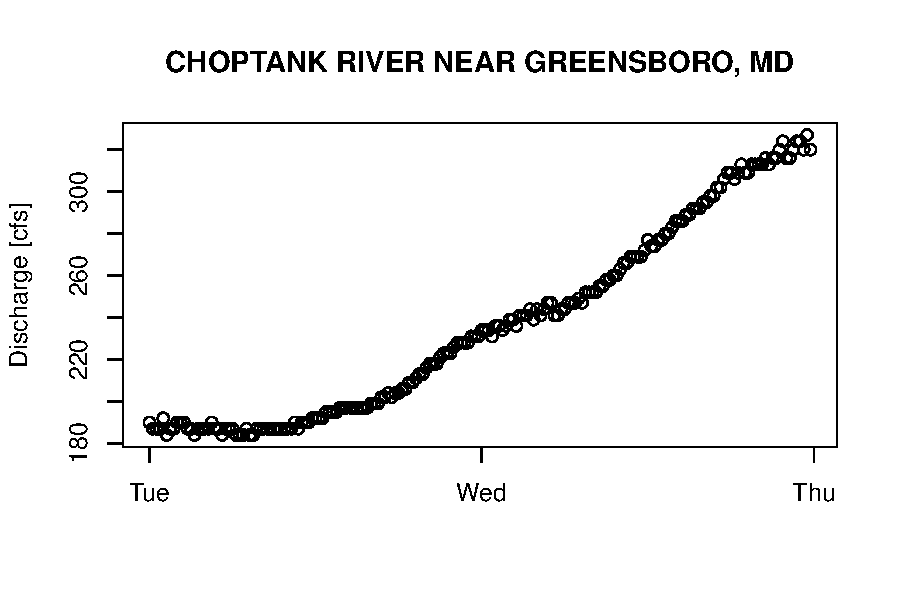
\includegraphics{dataRetrieval-fig2}
\end{center}
\caption{Real-time discharge plot of Choptank River.}
\end{figure}


%------------------------------------------------------------
\subsection{USGS Water Quality Retrievals}
%------------------------------------------------------------
Finally, we can use the dataRetrieval package to get USGS water quality data that is available on the water quality data portal: \url{http://www.waterqualitydata.us/}. The raw data us obtained from the function  getRawQWData, with the similar input arguments: siteNumber, parameterCd, startDate, endDate, and interactive. The difference is in parameterCd, in this function multiple parameters can be queried using a ";" separator, and setting parameterCd <- "" will return all of the measured observations. The raw data can be overwelming (as will be demonstrated), a simplified version of the data can be obtained using getQWData.


\begin{Schunk}
\begin{Sinput}
> siteNumber <- "01491000" 
> # Dissolved Nitrate parameter codes:
> parameterCd <- "00618;71851"  
> startDate <- "1964-06-11"
> endDate <- "2012-12-18"
> dissolvedNitrate <- getRawQWData(siteNumber, parameterCd, 
       startDate, endDate)
\end{Sinput}
\end{Schunk}

There is a large amount of data returned for each observation. The column names are listed below:


% latex table generated in R 2.15.2 by xtable 1.7-0 package
% Thu Feb 14 17:09:20 2013
\begin{tabular}{rll}
  \hline
 & ColumnNames & ColumnNames.1 \\ 
  \hline
1 & OrganizationIdentifier & CharacteristicName \\ 
  2 & OrganizationFormalName & ResultSampleFractionText \\ 
  3 & ActivityIdentifier & ResultMeasureValue \\ 
  4 & ActivityTypeCode & ResultMeasure.MeasureUnitCode \\ 
  5 & ActivityMediaName & MeasureQualifierCode \\ 
  6 & ActivityMediaSubdivisionName & ResultStatusIdentifier \\ 
  7 & ActivityStartDate & StatisticalBaseCode \\ 
  8 & ActivityStartTime.Time & ResultValueTypeName \\ 
  9 & ActivityStartTime.TimeZoneCode & ResultWeightBasisText \\ 
  10 & ActivityEndDate & ResultTimeBasisText \\ 
  11 & ActivityEndTime.Time & ResultTemperatureBasisText \\ 
  12 & ActivityEndTime.TimeZoneCode & ResultParticleSizeBasisText \\ 
  13 & ActivityDepthHeightMeasure.MeasureValue & PrecisionValue \\ 
  14 & ActivityDepthHeightMeasure.MeasureUnitCode & ResultCommentText \\ 
  15 & ActivityDepthAltitudeReferencePointText & USGSPCode \\ 
  16 & ActivityTopDepthHeightMeasure.MeasureValue & ResultDepthHeightMeasure.MeasureValue \\ 
  17 & ActivityTopDepthHeightMeasure.MeasureUnitCode & ResultDepthHeightMeasure.MeasureUnitCode \\ 
  18 & ActivityBottomDepthHeightMeasure.MeasureValue & ResultDepthAltitudeReferencePointText \\ 
  19 & ActivityBottomDepthHeightMeasure.MeasureUnitCode & SubjectTaxonomicName \\ 
  20 & ProjectIdentifier & SampleTissueAnatomyName \\ 
  21 & ActivityConductingOrganizationText & ResultAnalyticalMethod.MethodIdentifier \\ 
  22 & MonitoringLocationIdentifier & ResultAnalyticalMethod.MethodIdentifierContext \\ 
  23 & ActivityCommentText & ResultAnalyticalMethod.MethodName \\ 
  24 & SampleAquifer & MethodDescriptionText \\ 
  25 & HydrologicCondition & LaboratoryName \\ 
  26 & HydrologicEvent & AnalysisStartDate \\ 
  27 & SampleCollectionMethod.MethodIdentifier & ResultLaboratoryCommentText \\ 
  28 & SampleCollectionMethod.MethodIdentifierContext & DetectionQuantitationLimitTypeName \\ 
  29 & SampleCollectionMethod.MethodName & DetectionQuantitationLimitMeasure.MeasureValue \\ 
  30 & SampleCollectionEquipmentName & DetectionQuantitationLimitMeasure.MeasureUnitCode \\ 
  31 & ResultDetectionConditionText & PreparationStartDate \\ 
   \hline
\end{tabular}
\\*
To get a simplified dataframe that contains only datetime, value, and qualifier, use the function getQWData:

\begin{Schunk}
\begin{Sinput}
> dissolvedNitrateSimple <- getQWData(siteNumber, parameterCd, 
         startDate, endDate)
> names(dissolvedNitrateSimple)
\end{Sinput}
\begin{Soutput}
[1] "dateTime"        "qualifier.71851" "value.71851"     "qualifier.00618"
[5] "value.00618"    
\end{Soutput}
\end{Schunk}
Note that in this dataframe, datatime is imported as Dates (no times are included), and the qualifier is either blank or \verb@"<"@ signifying a censored value.

An example of plotting the above data (Figure 3):

\begin{Schunk}
\begin{Sinput}
> with(dissolvedNitrateSimple, plot(
   dateTime, value.00618,
   xlab="Date",ylab = paste(parameterINFO$srsname,
       "[",parameterINFO$parameter_units,"]")
   ))
\end{Sinput}
\end{Schunk}

\begin{figure}
\begin{center}
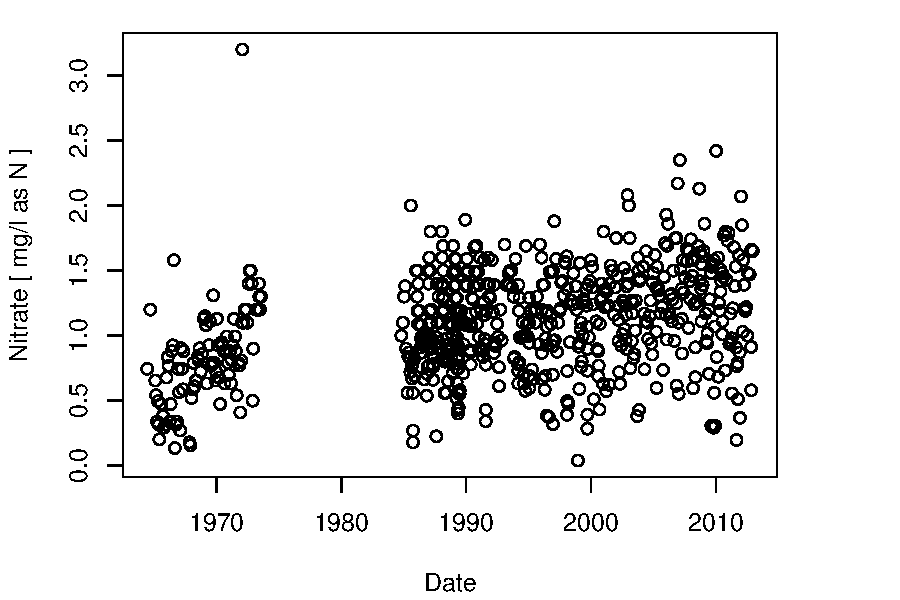
\includegraphics{dataRetrieval-fig3}
\end{center}
\caption{Nitrate plot of Choptank River.}
\end{figure}

%------------------------------------------------------------
\subsection{Other Water Quality Retrievals}
%------------------------------------------------------------
Additionally, there are additional data sets available on the Water Quality Portal (\url{http://www.waterqualitydata.us/}).  These data sets can be housed in either the STORET or NWIS database.  Since STORET does not use USGS parameter codes, a 'characteristic name' must be supplied.  The following example retrieves specific conductance from a DNR site in Wisconsin.

\begin{Schunk}
\begin{Sinput}
> specificCond <- getWQPData('WIDNR_WQX-10032762', 
         'Specific conductance', '', '')
> head(specificCond)
\end{Sinput}
\begin{Soutput}
    dateTime qualifier.Specific conductance value.Specific conductance
1 2011-02-14                                                      1360
2 2011-02-17                                                      1930
3 2011-03-03                                                      1240
4 2011-03-10                                                      1480
5 2011-03-29                                                      1130
6 2011-04-07                                                      1200
\end{Soutput}
\end{Schunk}


%------------------------------------------------------------
\section{Polished Data: USGS Web Retrieval Examples}
%------------------------------------------------------------ 
Rather than using the raw data as retrieved by the web, the dataRetrieval package also includes functions that return the data in a structure that has been designed to work with the EGRET R package (\url{https://github.com/USGS-R/EGRET/wiki}). In general, these dataframes may be much more 'R-friendly' than the raw data, and will contain additional date information that allows for efficient data analysis.

In this section, we use 3 dataRetrieval functions to get sufficient data to perform an EGRET analysis.  We will continue analyzing the Choptank River. We will need essentially the same data that was retrieved in the previous section, but we will get the daily discharge values in a dataframe called Daily, the nitrate sample data in a dataframe called Sample, and the data about the station and parameters in a dataframe called INFO. These are the dataframes that were exclusively designed to work with the EGRET R package, however can be very useful for all hydrologic studies.

%------------------------------------------------------------
\subsection{Daily Data}
%------------------------------------------------------------
The function to obtain the daily values (discharge in this case) is getDVData.  It requires the inputs siteNumber, ParameterCd, StartDate, EndDate, interactive, and convert. Most of these arguments are described in the previous section, however 'convert' is a new argument, it's default is TRUE, and it tells the program to convert the values from cfs to cms. If you don't want this conversion, set convert=FALSE in the function call.

\begin{Schunk}
\begin{Sinput}
> siteNumber <- "01491000"
> parameterCd <- "00631"  # Nitrate
> startDate <- "1964-01-01"
> endDate <- "2013-01-01"
> Daily <- getDVData(siteNumber, "00060", startDate, endDate,interactive=FALSE)
> summary(Daily)
\end{Sinput}
\begin{Soutput}
      Date                  Q                 Julian          Month       
 Min.   :1964-01-01   Min.   :  0.00991   Min.   :41637   Min.   : 1.000  
 1st Qu.:1976-04-01   1st Qu.:  0.87782   1st Qu.:46112   1st Qu.: 4.000  
 Median :1988-07-02   Median :  2.26535   Median :50586   Median : 7.000  
 Mean   :1988-07-02   Mean   :  4.01787   Mean   :50586   Mean   : 6.522  
 3rd Qu.:2000-10-01   3rd Qu.:  4.55901   3rd Qu.:55061   3rd Qu.:10.000  
 Max.   :2013-01-01   Max.   :246.35656   Max.   :59535   Max.   :12.000  
                                                                          
      Day           DecYear        MonthSeq     Qualifier        
 Min.   :  1.0   Min.   :1964   Min.   :1369   Length:17899      
 1st Qu.: 92.0   1st Qu.:1976   1st Qu.:1516   Class :character  
 Median :183.0   Median :1989   Median :1663   Mode  :character  
 Mean   :183.1   Mean   :1989   Mean   :1663                     
 3rd Qu.:274.0   3rd Qu.:2001   3rd Qu.:1810                     
 Max.   :366.0   Max.   :2013   Max.   :1957                     
                                                                 
       i              LogQ               Q7                Q30          
 Min.   :    1   Min.   :-4.6141   Min.   : 0.01808   Min.   : 0.09606  
 1st Qu.: 4476   1st Qu.:-0.1303   1st Qu.: 0.92232   1st Qu.: 1.05811  
 Median : 8950   Median : 0.8177   Median : 2.45143   Median : 2.83074  
 Mean   : 8950   Mean   : 0.7258   Mean   : 4.01655   Mean   : 4.01178  
 3rd Qu.:13424   3rd Qu.: 1.5171   3rd Qu.: 4.92309   3rd Qu.: 5.61594  
 Max.   :17899   Max.   : 5.5068   Max.   :84.00395   Max.   :25.47478  
                                   NA's   :6          NA's   :29        
\end{Soutput}
\end{Schunk}

Details of the Daily dataframe are listed below:

% latex table generated in R 2.15.2 by xtable 1.7-0 package
% Thu Feb 14 17:09:24 2013
\begin{tabular}{rlll}
  \hline
 & ColumnName & Type & Description \\ 
  \hline
1 & Date & Date & Date \\ 
  2 & Q & number & Discharge in cms \\ 
  3 & Julian & number & Number of days since January 1, 1850 \\ 
  4 & Month & integer & Month of the year [1-12] \\ 
  5 & Day & integer & Day of the year [1-366] \\ 
  6 & DecYear & number & Decimal year \\ 
  7 & MonthSeq & integer & Number of months since January 1, 1850 \\ 
  8 & Qualifier & string & Qualifing code \\ 
  9 & i & integer & Index \\ 
  10 & LogQ & number & Natural logarithm of Q \\ 
  11 & Q7 & number & 7 day running average of Q \\ 
  12 & Q30 & number & 30 running average of Q \\ 
   \hline
\end{tabular}\\*

The code will shift the discharge values to 0.001 times the mean if there are zero values detected in order to perform the logarithm. Columns Q7 and Q30 are 7 and 30 day running averages. 

%------------------------------------------------------------
\subsection{Sample Data}
%------------------------------------------------------------
The function to obtain sample data from the water quality portal is getSampleData. The arguments for this function are also siteNumber, ParameterCd, StartDate, EndDate, interactive. These are the same inputs as getRawQWData or getQWData as described in the previous section.

\begin{Schunk}
\begin{Sinput}
> Sample <-getSampleData(siteNumber,parameterCd,
       startDate, endDate,interactive=FALSE)
> summary(Sample)
\end{Sinput}
\begin{Soutput}
      Date               ConcLow         ConcHigh         Uncen       
 Min.   :1973-06-04   Min.   :0.176   Min.   :0.050   Min.   :0.0000  
 1st Qu.:1989-01-31   1st Qu.:0.900   1st Qu.:0.900   1st Qu.:1.0000  
 Median :1995-02-15   Median :1.150   Median :1.150   Median :1.0000  
 Mean   :1996-04-07   Mean   :1.145   Mean   :1.143   Mean   :0.9984  
 3rd Qu.:2003-08-26   3rd Qu.:1.400   3rd Qu.:1.400   3rd Qu.:1.0000  
 Max.   :2012-12-18   Max.   :2.430   Max.   :2.430   Max.   :1.0000  
                      NA's   :1                                       
    ConcAve          Julian          Month             Day       
 Min.   :0.025   Min.   :45079   Min.   : 1.000   Min.   :  2.0  
 1st Qu.:0.900   1st Qu.:50799   1st Qu.: 3.000   1st Qu.: 81.0  
 Median :1.150   Median :53005   Median : 6.000   Median :161.0  
 Mean   :1.143   Mean   :53423   Mean   : 6.155   Mean   :170.7  
 3rd Qu.:1.400   3rd Qu.:56119   3rd Qu.: 9.000   3rd Qu.:261.0  
 Max.   :2.430   Max.   :59521   Max.   :12.000   Max.   :363.0  
                                                                 
    DecYear        MonthSeq        SinDY              CosDY         
 Min.   :1973   Min.   :1482   Min.   :-1.00000   Min.   :-0.99996  
 1st Qu.:1989   1st Qu.:1670   1st Qu.:-0.65358   1st Qu.:-0.66655  
 Median :1995   Median :1742   Median : 0.16237   Median : 0.03433  
 Mean   :1996   Mean   :1756   Mean   : 0.06474   Mean   : 0.02331  
 3rd Qu.:2004   3rd Qu.:1844   3rd Qu.: 0.76785   3rd Qu.: 0.72212  
 Max.   :2013   Max.   :1956   Max.   : 0.99985   Max.   : 0.99967  
\end{Soutput}
\end{Schunk}

Details of the Sample dataframe are listed below:

% latex table generated in R 2.15.2 by xtable 1.7-0 package
% Thu Feb 14 17:09:25 2013
\begin{tabular}{rlll}
  \hline
 & ColumnName & Type & Description \\ 
  \hline
1 & Date & Date & Date \\ 
  2 & ConcLow & number & Lower limit of concentration \\ 
  3 & ConcHigh & number & Upper limit of concentration \\ 
  4 & Uncen & integer & Uncensored data (1=true, 0=false) \\ 
  5 & ConcAve & number & Average concentration \\ 
  6 & Julian & number & Number of days since January 1, 1850 \\ 
  7 & Month & integer & Month of the year [1-12] \\ 
  8 & Day & integer & Day of the year [1-366] \\ 
  9 & DecYear & number & Decimal year \\ 
  10 & MonthSeq & integer & Number of months since January 1, 1850 \\ 
  11 & SinDY & number & Sine of ... \\ 
  12 & CosDY & number & Cosine of ... \\ 
  13 & Q & number & Discharge in cms \\ 
  14 & LogQ & number & Natural logarithm of flow \\ 
   \hline
\end{tabular}
In a more complex situation, the Sample data frame will combine all of the measured parameters.  An example is provided to explain how the values are combined:

%------------------------------------------------------------
\subsection{Complex Sample Data Example}
%------------------------------------------------------------
As an example, let us say that in 2004 and earlier, we computed a total phosphorus (tp) as the sum of dissolved phosphorus (dp) and particulate phosphorus (pp). Form 2005 and onward, we have direct measurements of total phosphorus (tp). A small subset of this fictional data looks like this:

% latex table generated in R 2.15.2 by xtable 1.7-0 package
% Thu Feb 14 17:09:25 2013
\begin{tabular}{rllrlrlr}
  \hline
 & cdate & rdp & dp & rpp & pp & rtp & tp \\ 
  \hline
1 & 2003-02-15 &  & 0.02 &  & 0.50 &  &  \\ 
  2 & 2003-06-30 & $<$ & 0.01 &  & 0.30 &  &  \\ 
  3 & 2004-09-15 & $<$ & 0.00 & $<$ & 0.20 &  &  \\ 
  4 & 2005-01-30 &  &  &  &  &  & 0.43 \\ 
  5 & 2005-05-30 &  &  &  &  & $<$ & 0.05 \\ 
  6 & 2005-10-30 &  &  &  &  & $<$ & 0.02 \\ 
   \hline
\end{tabular}\\*

The dataRetrieval package will "add up" all the values in a given row to form the total for that sample. Thus, you only want to enter data that should be added together. For example, we might know the value for dp on 5/30/2005, but we don't want to put it in the table because under the rules of this data set, we are not suppose to add it in to the values in 2005.

For every sample, the EGRET package requires a pair of numbers to define an interval in which the true value lies (ConcLow and ConcHigh). In a simple non-censored case (the reported value is above the detection limit), ConcLow equals ConcHigh and the interval collapses down to a single point.In a simple censored case, the value might be reported as <0.2, then ConcLow=NA and ConcHigh=0.2. We use NA instead of 0 as a way to elegantly handle future logarithm calculations.

For the more complex example case, let us say dp is reported as <0.01 and pp is reported as 0.3. We know that the total must be at least 0.3 and could be as much as 0.31. Therefore, ConcLow=0.3 and ConcHigh=0.31. Another case would be if dp is reported as <0.005 and pp is reported <0.2. We know in this case that the true value could be as low as zero, but could be as high as 0.205. Therefore, in this case, ConcLow=NA and ConcHigh=0.205. The Sample dataframe for the example data is therefore:

\begin{Schunk}
\begin{Soutput}
        Date ConcLow ConcHigh Uncen ConcAve Julian Month Day  DecYear MonthSeq
1 2003-02-15    0.52    0.520     1  0.5200  55927     2  46 2003.124     1838
2 2003-06-30    0.30    0.310     0  0.3050  56062     6 181 2003.493     1842
3 2004-09-15      NA    0.205     0  0.1025  56505     9 259 2004.706     1857
4 2005-01-30    0.43    0.430     1  0.4300  56642     1  30 2005.081     1861
5 2005-05-30      NA    0.050     0  0.0250  56762     5 150 2005.408     1865
6 2005-10-30      NA    0.020     0  0.0100  56915    10 303 2005.827     1870
        SinDY      CosDY
1  0.70406552  0.7101350
2  0.04290476 -0.9990792
3 -0.96251346 -0.2712339
4  0.48505985  0.8744810
5  0.54391895 -0.8391378
6 -0.88668032  0.4623830
\end{Soutput}
\end{Schunk}



%------------------------------------------------------------
\subsection{INFO Data}
%------------------------------------------------------------
The function to obtain "metadata", data about the gage station and measured parameters is getMetaData. This function essentially combines getSiteFileData and getParameterInfo, producing one dataframe called INFO.

\begin{Schunk}
\begin{Sinput}
> INFO <-getMetaData(siteNumber,parameterCd, interactive=FALSE)
\end{Sinput}
\end{Schunk}

Column names in the INFO dataframe are listed below:

% latex table generated in R 2.15.2 by xtable 1.7-0 package
% Thu Feb 14 17:09:26 2013
\begin{tabular}{rll}
  \hline
 & ColumnNames & ColumnNames.1 \\ 
  \hline
1 & agency.cd & alt.datum.cd \\ 
  2 & site.no & huc.cd \\ 
  3 & station.nm & basin.cd \\ 
  4 & site.tp.cd & topo.cd \\ 
  5 & lat.va & construction.dt \\ 
  6 & long.va & inventory.dt \\ 
  7 & dec.lat.va & drain.area.va \\ 
  8 & dec.long.va & contrib.drain.area.va \\ 
  9 & coord.meth.cd & tz.cd \\ 
  10 & coord.acy.cd & local.time.fg \\ 
  11 & coord.datum.cd & reliability.cd \\ 
  12 & dec.coord.datum.cd & project.no \\ 
  13 & district.cd & queryTime \\ 
  14 & state.cd & drainSqKm \\ 
  15 & county.cd & staAbbrev \\ 
  16 & country.cd & param.nm \\ 
  17 & map.nm & param.units \\ 
  18 & map.scale.fc & paramShortName \\ 
  19 & alt.va & paramNumber \\ 
  20 & alt.meth.cd & constitAbbrev \\ 
  21 & alt.acy.va &  \\ 
   \hline
\end{tabular}
\\*


\newpage
%------------------------------------------------------------ 
\section{Retrieving User-Generated Data Files}
%------------------------------------------------------------ 
Aside from retrieving data from the USGS web services, the dataRetrieval package includes functions to generate the Daily and Sample data frame from local files.

%------------------------------------------------------------ 
\subsection{getDailyDataFromFile}
%------------------------------------------------------------ 
getDailyDataFromFile will load a user-supplied text file and convert it to the Daily dataframe. The file should have two columns, the first dates, the second values.  The dates should be formatted either mm/dd/yyyy or yyyy-mm-dd. Using a 4-digit year is required. This function has the following inputs: filePath, fileName,hasHeader (TRUE/FALSE), separator, qUnit, and interactive (TRUE/FALSE). filePath is a string that defines the path to your file. This can either be a full path, or path relative to your R working directory. The input fileName is a string that defines the file name (including the extension).

Text files that contain this sort of data require some sort of a separator, for example, a 'csv' file (aka 'comma-separated value') file uses a comma to separate the date and value column. A tab delimited file would use a tab ("\verb@\t@") rather than the comma (","). The type of separator you use can be defined in the function call in the 'separator' argument, the default is ",". Another function input is a logical variable: hasHeader.  The default is TRUE. If your data does not have column names, set this variable to FALSE.

Finally, qUnit is a numeric input that defines the discharge/flow units. Flow from the NWIS web results are typically given in cubic feet per second (qUnit=1), but the EGRET package requires flow to be given in cubic meters per second (qUnit=2). Other allowed values are 10\verb@^@3 cubic feet per second (qUnit=3) and 10\verb@^@3 cubic meters per second (qUnit=4). If you do not want your data to be converted, use qUnit=2. The default is qUnit=1 (assumes flow is in cubic feet per second).

So, if you have a file called "ChoptankRiverFlow.txt" located in a folder called "RData" on your C drive (this is a Window's example), and the file is structured as follows (tab-separated):
\begin{verbatim}
date  Qdaily
10/1/1999  3.029902561
10/2/1999	2.406931941
10/3/1999	2.152080324
10/4/1999	2.152080324
10/5/1999	3.19980364
10/6/1999	2.775050944
...
\end{verbatim}

The call to open this file, convert the flow to cubic meters per second, and populate the Daily data frame would be:
\begin{Schunk}
\begin{Sinput}
> fileName <- "ChoptankRiverFlow.txt"
> filePath <-  "~/RData/"
> Daily <- getDailyDataFromFile(filePath,fileName,separator="\t",interactive=FALSE)
> head(Daily)
\end{Sinput}
\begin{Soutput}
        Date          Q Julian Month Day  DecYear MonthSeq i      LogQ Q7 Q30
1 1999-10-01 0.08579729  54694    10 274 1999.747     1798 1 -2.455768 NA  NA
2 1999-10-02 0.06815672  54695    10 275 1999.750     1798 2 -2.685945 NA  NA
3 1999-10-03 0.06094013  54696    10 276 1999.753     1798 3 -2.797863 NA  NA
4 1999-10-04 0.06094013  54697    10 277 1999.755     1798 4 -2.797863 NA  NA
5 1999-10-05 0.09060835  54698    10 278 1999.758     1798 5 -2.401209 NA  NA
6 1999-10-06 0.07858069  54699    10 279 1999.761     1798 6 -2.543629 NA  NA
\end{Soutput}
\end{Schunk}

%------------------------------------------------------------ 
\subsection{getSampleDataFromFile}
%------------------------------------------------------------ 
Similarly to the previous section, getSampleDataFromFile will import a user-generated file and populate the Sample dataframe. The difference between sample data and flow data is that the code requires a third column that contains a remark code, either blank or \verb@"<"@, which will tell the program that the data was 'left-censored' (or, below the detection limit of the sensor). Therefore, the data is required to be in the form: date, remark, value.  If multiple constituents are going to be used, the format can be date, remark\_A, value\_A, remark\_b, value\_b, etc... An example of a comma-delimited file would be:

\begin{verbatim}
cdate;remarkCode;Nitrate
10/7/1999,,1.4
11/4/1999,<,0.99
12/3/1999,,1.42
1/4/2000,,1.59
2/3/2000,,1.54
...
\end{verbatim}
The call to open this file, and populate the Sample dataframe would be:
\begin{Schunk}
\begin{Sinput}
> fileName <- "ChoptankRiverNitrate.csv"
> filePath <-  "C:/RData/"
> Sample <- getSampleDataFromFile(filePath,fileName,separator=",",interactive=FALSE)
> head(Sample)
\end{Sinput}
\begin{Soutput}
        Date ConcLow ConcHigh Uncen ConcAve Julian Month Day  DecYear MonthSeq
1 1999-10-07    1.40     1.40     1   1.400  54700    10 280 1999.764     1798
2 1999-11-04      NA     0.99     0   0.495  54728    11 308 1999.840     1799
3 1999-12-03    1.42     1.42     1   1.420  54757    12 337 1999.919     1800
4 2000-01-04    1.59     1.59     1   1.590  54789     1   4 2000.010     1801
5 2000-02-03    1.54     1.54     1   1.540  54819     2  34 2000.092     1802
6 2000-02-15    1.37     1.37     1   1.370  54831     2  46 2000.124     1802
        SinDY     CosDY
1 -0.99631836 0.0857305
2 -0.84377556 0.5366962
3 -0.48505985 0.8744810
4  0.06004896 0.9981954
5  0.54391895 0.8391378
6  0.70406552 0.7101350
\end{Soutput}
\end{Schunk}


\newpage
%------------------------------------------------------------ 
\section{Appendix 1: Getting Started}
%------------------------------------------------------------ 
This section describes the options for downloading and installing the dataRetrieval package.

%------------------------------------------------------------
\subsection{New to R?}
%------------------------------------------------------------ 
If you are new to R, you will need to first install the latest version of R, which can be found here: \url{http://www.r-project.org/}.

There are many options for running and editing R code, one nice enviornment to learn R is RStudio. RStudio can be downloaded here: \url{http://rstudio.org/}. Once R and RStudio are installed, the dataRetrieval package needs to be installed as described in the next section.

%------------------------------------------------------------
\subsection{R User: Installing dataRetrieval from downloaded binary}
%------------------------------------------------------------ 
The latest dataRetrieval package build is available for download at \url{https://github.com/USGS-R/dataRetrieval/blob/master/dataRetrieval_1.2.1.tar.gz}.  If the package's tar.gz file is saved in R's working directory, then the following command will fully install the package:

\begin{Schunk}
\begin{Sinput}
> install.packages("dataRetrieval_1.2.1.tar.gz", 
                  repos=NULL, type="source")
\end{Sinput}
\end{Schunk}

If the downloaded file is stored in an alternative location, include the path in the install command.  A Windows example looks like this (notice the direction of the slashes, they are in the opposite direction that Windows normally creates paths):

\begin{Schunk}
\begin{Sinput}
> install.packages(
   "C:/RPackages/Statistics/dataRetrieval_1.2.1.tar.gz", 
   repos=NULL, type="source")
\end{Sinput}
\end{Schunk}

A Mac example looks like this:

\begin{Schunk}
\begin{Sinput}
> install.packages(
   "/Users/userA/RPackages/Statistic/dataRetrieval_1.2.1.tar.gz", 
   repos=NULL, type="source")
\end{Sinput}
\end{Schunk}

It is a good idea to re-start the R enviornment after installing the package, especially if installing an updated version (that is, restart RStudio). Some users have found it necessary to delete the previous version's package folder before installing newer version of dataRetrieval. If you are experiencing issues after updating a package, trying deleting the package folder - the default location for Windows is something like this: C:/Users/userA/Documents/R/win-library/2.15/dataRetrieval, and the default for a Mac: /Users/userA/Library/R/2.15/library/dataRetrieval. Then, re-install the package using the directions above. Moving to CRAN should solve this problem.

After installing the package, you need to open the library each time you re-start R.  This is done with the simple command:
\begin{Schunk}
\begin{Sinput}
> library(dataRetrieval)
\end{Sinput}
\end{Schunk}
Using RStudio, you could alternatively click on the checkbox for dataRetrieval in the Packages window.

%------------------------------------------------------------
\subsection{R Developers: Installing dataRetrieval from gitHub}
%------------------------------------------------------------
Alternatively, R-developers can install the latest version of dataRetrieval directly from gitHub using the devtools package.  devtools is available on CRAN.  Simpley type the following commands into R to install the latest version of dataRetrieval available on gitHub.  Rtools (for Windows) and appropriate \LaTeX\ tools are required.

\begin{Schunk}
\begin{Sinput}
> library(devtools)
> install_github("dataRetrieval", "USGS-R")
\end{Sinput}
\end{Schunk}
To then open the library, simply type:

\begin{Schunk}
\begin{Sinput}
> library(dataRetrieval)
\end{Sinput}
\end{Schunk}

\newpage


%------------------------------------------------------------
% BIBLIO
%------------------------------------------------------------
\begin{thebibliography}{10}

\bibitem{HirschI}
Helsel, D.R. and R. M. Hirsch, 2002. Statistical Methods in Water Resources Techniques of Water Resources Investigations, Book 4, chapter A3. U.S. Geological Survey. 522 pages. \url{http://pubs.usgs.gov/twri/twri4a3/}

\bibitem{HirschII}
Hirsch, R. M., Moyer, D. L. and Archfield, S. A. (2010), Weighted Regressions on Time, Discharge, and Season (WRTDS), with an Application to Chesapeake Bay River Inputs. JAWRA Journal of the American Water Resources Association, 46: 857-880. doi: 10.1111/j.1752-1688.2010.00482.x \url{http://onlinelibrary.wiley.com/doi/10.1111/j.1752-1688.2010.00482.x/full}

\bibitem{HirschIII}
Sprague, L. A., Hirsch, R. M., and Aulenbach, B. T. (2011), Nitrate in the Mississippi River and Its Tributaries, 1980 to 2008: Are We Making Progress? Environmental Science \& Technology, 45 (17): 7209-7216. doi: 10.1021/es201221s \url{http://pubs.acs.org/doi/abs/10.1021/es201221s}

\end{thebibliography}

\end{document}

\end{document}
